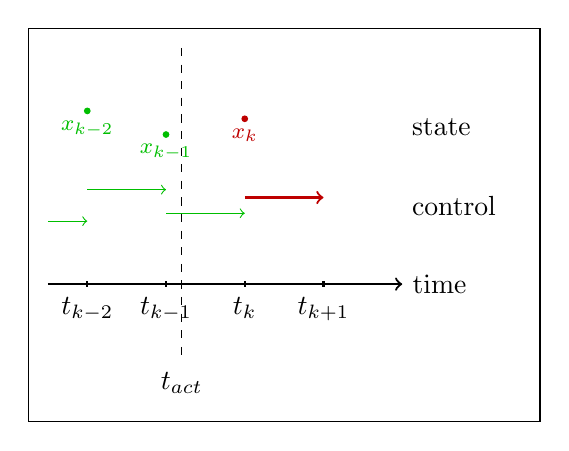
\begin{tikzpicture}
\definecolor{green}{RGB}{0,190,0};
\definecolor{red}{RGB}{190,0,0};

%Draw bounding box
\draw (-2.75,-1.75) rectangle (3.75,3.25);

%Draw time line
\draw[ thick, ->] (-2.5,0) -- (2,0) node[anchor=west] {time};
\foreach  \t in  {-2, -1, +1}
	\draw[thick]  (\t cm, 1pt)  -- (\t cm, -1pt) node[anchor=north] {$t_{k \t  }$ };
\draw[thick]  (0cm , 1pt)  -- (0 cm, -1pt) node[anchor=north] {$t_k$ };

%draw known controls
\draw (2,1) node[anchor=west] {control};
\draw[->,green] (-2.5, 0.8) -- (-2,0.8) ;
\draw[->,green] (-2, 1.2) -- (-1,1.2) ;
\draw[->,green] (-1, 0.9) -- (0,0.9) ;
\draw[->,red,thick] (0, 1.1) -- (1,1.1) ;

%Draw actual time
\draw[dashed] (-.8,3) -- (-.8,-1) node[anchor=north] {$t_{act}$};

%Draw exact states
\draw (2,2) node[anchor=west] {state};
\draw[green, fill=green] (-2, 2.2) circle (1pt) node[anchor=north]{\footnotesize $x_{k-2}$};
\draw[green, fill=green] (-1, 1.9) circle (1pt) node[anchor=north]{\footnotesize $x_{k-1}$};
\draw[red, fill=red] (0,2.1) circle (1pt) node[anchor=north]{\footnotesize $x_{k}$};
\end{tikzpicture}